\section{Semantic application queries}

\subsubsection{An alternative presentation}

If you recall, there's an alternative way to present monads that are
algebras, like our monoid monad. Algebras are presented in terms of
generators and relations. In our case the generators presentation is
really just a grammar for monoid expressions.

\begin{mathpar}
  \inferrule* [lab=expression] {} {{m,n} ::=}
  \and
  \inferrule* [lab=identity element] {} {e}
  \and
  \inferrule* [lab=generators] {} {\;| \; g_1 \; | \; ... \; | \; g_n}
  \and
  \inferrule* [lab=monoid-multiplication] {} {\;| \; m * n}
\end{mathpar} 

This is subject to the following constraints, meaning that we will
treat syntactic expressions of certain forms as denoting the same
element of the monoid. To emphasize the nearly purely syntactic role
of these constraints we will use a different symbol for the
constraints. We also use the same symbol, $\equiv$, for the smallest equivalence
relation respecting these constraints.

\begin{mathpar}
  \inferrule* [lab=identity laws] {} {m * e \equiv m \equiv e * m}
  \and
  \inferrule* [lab=associativity] {} {m_1 * (m_2 * m_3) \equiv (m_1 * m_2) * m_3}
\end{mathpar} 

\paragraph{Logic: the set monad as an algebra}
In a similar manner, there is a language associated with the monad of
sets \emph{considered as an algebra}. This language is very familiar
to most programmers.

\begin{mathpar}
  \inferrule* [lab=expression] {} {{c,d} ::=}
  \and
  \inferrule* [lab=identity verity] {} {true}
  \and
  \inferrule* [lab=negation] {} {\;| \; \neg c}
  \and
  \inferrule* [lab=conjunction] {} {\;| \; c \& d}
\end{mathpar} 

Now, if we had a specific set in hand, say $L$ (which we'll call a
universe in the sequel), we can interpret the expressions in the this
language, aka formulae, in terms of operations on subsets of that
set. As with our compiler for the concrete syntax of the
$lambda$-calculus in chapter 1, we can express this translation very
compactly as

\begin{mathpar}
  \inferrule* {} {\meaningof{true} = L}
  \and
  \inferrule* {} {\meaningof{\neg c} = L \backslash c}
  \and 
  \inferrule* {} {\meaningof{c \& d} = \meaningof{c} \cap \meaningof{d}}
\end{mathpar}

Now, what's happening when we pull the monoid monad through the set
monad via a distributive map is this. First, the monoid monad
furnishes the universe, $L$, as the set of expressions generated by
the grammar. We'll denote this by $L(m)$. Then, we enrich the set of
formulae by the operations of the monoid \emph{acting on sets}.

\begin{mathpar}
  \inferrule* [lab=expression] {} {{c,d} ::=}
  \and
  \inferrule* [lab=identity verity] {} {true}
  \and
  \inferrule* [lab=negation] {} {\;| \; \neg c}
  \and
  \inferrule* [lab=conjunction] {} {\;| \; c \& d}
  \and
  \inferrule* [lab=identity verity] {} { \bf{e} }
  \and
  \inferrule* [lab=negation] {} {\;| \; \bf{g_1} \; | \; ... \; | \; \bf{g_n}}
  \and
  \inferrule* [lab=conjunction] {} {\;| \; c * d}
\end{mathpar} 

The identity element, $e$ and the generators of the monoid, $g_1$,
..., $g_n$, can be considered $0$-ary operations in the same way that
we usually consider constants as $0$-ary operations. To avoid
confusion between these elements and the \emph{logical formulae} that
pick them out of the crowd, we write the logical formulae in
$\bf{boldface}$.

Now, we can write our distributive map. Surprisingly, it is exactly a
meaning for our logic!

\begin{mathpar}
  \inferrule* {} {\meaningof{true} = L(m)}
  \and
  \inferrule* {} {\meaningof{\neg c} = L(m) \backslash c}
  \and 
  \inferrule* {} {\meaningof{c \& d} = \meaningof{c} \cap \meaningof{d}}
  \and
  \inferrule* {} {\meaningof{\bf{e}} = \{ m \; \in \; L(m) \; | \; m \equiv e \}}
  \and
  \inferrule* {} {\meaningof{\bf{g_i}} = \{ m \; \in \; L(m) \; | \; m \equiv g_i \}}
  \and
  \inferrule* {} {\meaningof{c*d} = \{ m \; \in \; L(m) \; | \; m \equiv m_1 * m_2, m_1 \; \in \; \meaningof{c}, m_2 \; \in \; \meaningof{d} \}}
\end{mathpar}

\paragraph{Primes: an application}
Before going any further, let's look at an example of how to use these
new operators. Suppose we wanted to pick out all the elements of the
monoid that were not expressible as a composition of other
elements. Obviously, for monoids with a finite set of generators, this
is exactly just the generators, so we could write $\bf{g_1} || ... ||
\bf{g_n}$\footnote{We get the disjunction, $||$, by the usual DeMorgan
  translation: $c || d \stackrel{def}{=} \neg( \neg c \& \neg
  d)$}. However, when the set of generators is not finite, as it is
when the monoid is the integers under multiplication, we need another
way to write this down. That's where our other operators come in
handy. A moment's thought suggests that we could say that since $true$
denotes any possible element in the monoid, an element is not a
composition using negation plus our composition formula, i.e. $\neg
(true * true)$. This is a little overkill, however. We just want to
eliminate non-trivial compositions. We know how to express the
identity element, that's $\bf{e}$, so we are interested in those
elements that are not the identity, i.e. $\neg \bf{e}$. Then a formula
that eliminates compositions of non-trivial elements is spelled out
$\neg (\neg e * \neg e)$ \footnote{Note the similarity of this
  construction to the DeMorgan construction of Boolean
  disjunction. This is, in fact, another kind of
  disjunction.}. Finally, we want to eliminate the identity as a
solution. So, we arrive at $\neg (\neg e * \neg e) \& \neg e$. There,
that formula picks out the \emph{primes} of \emph{any} monoid.

\paragraph{Summary}

What have we done? We've illustrated a specific distributive map, one
that pulls the set monad through the monoid monad. We've shown that
this particular distributive map coincides with giving a semantics to
a particular logic, one whose structure is derived solely from the
shape of the collection monad, i.e. set, and the shape of the term
language, in this case monoid.

The observation that the distributive map is also a semantics for a
logic comes about through a kind of factoring. We note that there is a
language, the language of Boolean algebra, that takes its meaning in
the set monad. As with the monoid monad, the \emph{syntax} of Boolean
algebra is given by a monad. The semantics of Boolean algebra can
expressed in terms of sets. That is, one can find models for the
syntax in terms of sets. In some sense, the distributive map is the
unique extension of that semantics map to an enrichment of the syntax
with the constructors of the monoid term language.

\subsubsection{Patterns}

The constructions of a language of patterns for our monoid expressions
is also completely determined by monadic structure. All we are really
doing is constructing the data type of 1-holed contexts. In chapter 6
we showed how the derivative of a given regular data type is exactly
the 1-holed contexts for the data type. This provides our first
example of how to calculate the pattern language for our
\lstinline[language=Scala,mathescape=true]!for!-comprehensions. After
calculation we arrive at

\begin{mathpar}
  \inferrule* [lab=expression] {} {{m,n} ::=}
  \and
  \inferrule* [lab=hole] {} {x}
  \and
  \inferrule* [lab=identity] {} {\;|\;e}
  \and

  \inferrule* [lab=generators] {} {\;| \; g_1 \; | \; ... \; | \; g_n}
  \and
  \inferrule* [lab=multiplication] {} {\;| \; m * n}
\end{mathpar} 

In some sense, the story here, much like the Sherlock Holmes story, is
that the dog didn't bark. The patterns we calculate from our term
language are precisely the sorts of patterns we expect if we modeled
our term language via \texttt{Scala}
\lstinline[language=Scala,mathescape=true]!case! classes.

\subsubsection{A first mini-query language}

We can now use these pieces to flesh out some examples of the kinds of
queries we might build. The expression

\begin{lstlisting}[language=Scala,mathescape=true]
  for( x <- d if $\neg (\neg e * \neg e) \& \neg e$ ) yield x
\end{lstlisting}

will result in a collection of primes residing in the data source
\lstinline[language=Scala,mathescape=true]!d!.

\begin{lstlisting}[language=Scala,mathescape=true]
  for( x <- d if $(\neg e * g)$ ) yield x
\end{lstlisting}

will result in a collection of expressions residing in the data source
\lstinline[language=Scala,mathescape=true]!d! having $g$ as a factor
in a non-trivial composition.

\subsubsection{Iterating the design pattern}

The whole point of working in this manner is that by virtue of its
compositional structure it provides a much higher level of abstraction
and greater opportunities for reuse. To illustrate the point, we will
now iterate the construction using our toy language, the
$lambda$-calculus, as the term language. As we saw in chapter 1, the
$lambda$-calculus also has a generators and relations
presentation. Unlike a monoid, however, the lambda calculus has
another piece of machinery: reduction! In addition to structural
equivalence of terms (which is a bi-directional relation) there is the
$beta$-reduction rule that captures the \emph{behavioral} aspect of
the lambda calculus.

It is key to understand this underlying structure of language
definitions. In essence, when a DSL is purely about structure it is
presented entirely in terms of generators (read: a grammar) and
relations (like the monoid laws). When the DSL is also about behavior,
i.e. the terms in the language somehow express some kind of
computation, then the language has a third component, some kind of
reduction relation. \footnote{In some sense this is one of the central
  contributions of the theory of computation back to
  mathematics. Algebraists have known for a long time about generators
  and relations presentations of algebraic structures (of which
  algebraic data types are a subset). This collective wisdom is
  studied, for example, in the field of universal
  algebra. Computational models like the $lambda$-calculus and more
  recently the process calculi, like Milner's $\pi$-calculus or
  Cardelli and Gordon's ambient calculus, take this presentation one
  step further and add a set of conditional rewrite rules to express
  the computational content of the model. It was Milner who first
  recognized this particular decomposition of language definitions in
  his seminal paper, Functions as Processes, where he reformulated the
  presentation $\pi$-calculus along these lines.} This organization,
this common factoring of the specification of a language, makes it
possible to factor code that handles a wide range of semantic
features. The logic we derive below provides a great example.

\paragraph{A spatial-behavioral-style logic for $\lambda$-calculus}

\begin{mathpar}
  \inferrule* [lab=expression] {} {{c,d} ::=}
  \and
  \inferrule* [lab=identity verity] {} {true}
  \and
  \inferrule* [lab=negation] {} {\;| \; \neg c}
  \and
  \inferrule* [lab=conjunction] {} {\;| \; c \& d}
  \\
  \inferrule* [lab=mention] {} {\; | \; \bf{x}}
  \and
  \inferrule* [lab=abstraction] {} {\;| \; \texttt{(} \bf{x_1} \texttt{,} ... \texttt{,} \bf{x_k} \texttt{)} \; \texttt{=>} \; c}
  \and
  \inferrule* [lab=application] {} {\;| \; c\texttt{(} c_1 \texttt{,} ... \texttt{,} c_k \texttt{)}}
  \\
  \inferrule* [lab=let] {} {\;| \; \texttt{\bf{val}} \; \bf{x} \; \texttt{\bf{=}} \; c \texttt{;} d}
  \and
  \inferrule* [lab=seq] {} {\;| \; c \texttt{;} d }
  \and
  \inferrule* [lab=group] {} {\;| \; \texttt{ \{ } c \texttt{ \} } }
  \\
  \inferrule* [lab=probe] {} {\;| \; \langle d \rangle c }
\end{mathpar} 

The first category of formulae, included for completeness, is again,
just the language of Boolean algebra we get because our collection
monad is \lstinline[language=Scala,mathescape=true]!Set!. The next
category comes directly from the abstract syntax of the
$\lambda$-calculus. The next group is of interest because it shows
that the construction faithfully supports syntactic sugar. The
semantics of the ``sugar'' formulae is the semantics of desugaring
factored through our distributive map. These latter two categories
allow us to investigate the structure of terms. The final category of
formulae, which has only one entry, $PROBE$, is the means of
investigating behavior of terms.

\paragraph{Examples}
Before we get to the formal specification of the semantics of our
logic, let's exercise intuition via a few examples.

\begin{itemize}
  \item \begin{lstlisting}[language=Scala,mathescape=true]
      for( fn( _, ..., _ ) <- d if $true( c_1, ..., c_n )$ ) yield fn
    \end{lstlisting}

  \item \begin{lstlisting}[language=Scala,mathescape=true]
      for( _( fixpt ) <- d
           if $(( f ) => (( x ) => f( x( x ) ))(( x ) => f( x( x ))))( true )$ )
      yield fixpt
    \end{lstlisting}
  \item \begin{lstlisting}[language=Scala,mathescape=true]
      for( a <- d if $\langle ( x ) => ((Y f) x) \rangle$ $\bf{a}$ )
      yield a
    \end{lstlisting}
\end{itemize}

The first of these will return the expressions in ``function''
position applied the actual parameters meeting the conditions
\lstinline[language=Scala,mathescape=true]!c$_i$! respectively. The
second will return all actual parameters of expressions that calculate
fixpoints. Both of these examples are representative common code
optimization schemes that are usually carefully hand-coded. The third
example finds all elements in d that are already fixpoints of a given
function, $f$.

\begin{figure}[tbp]
\begin{center}
{ 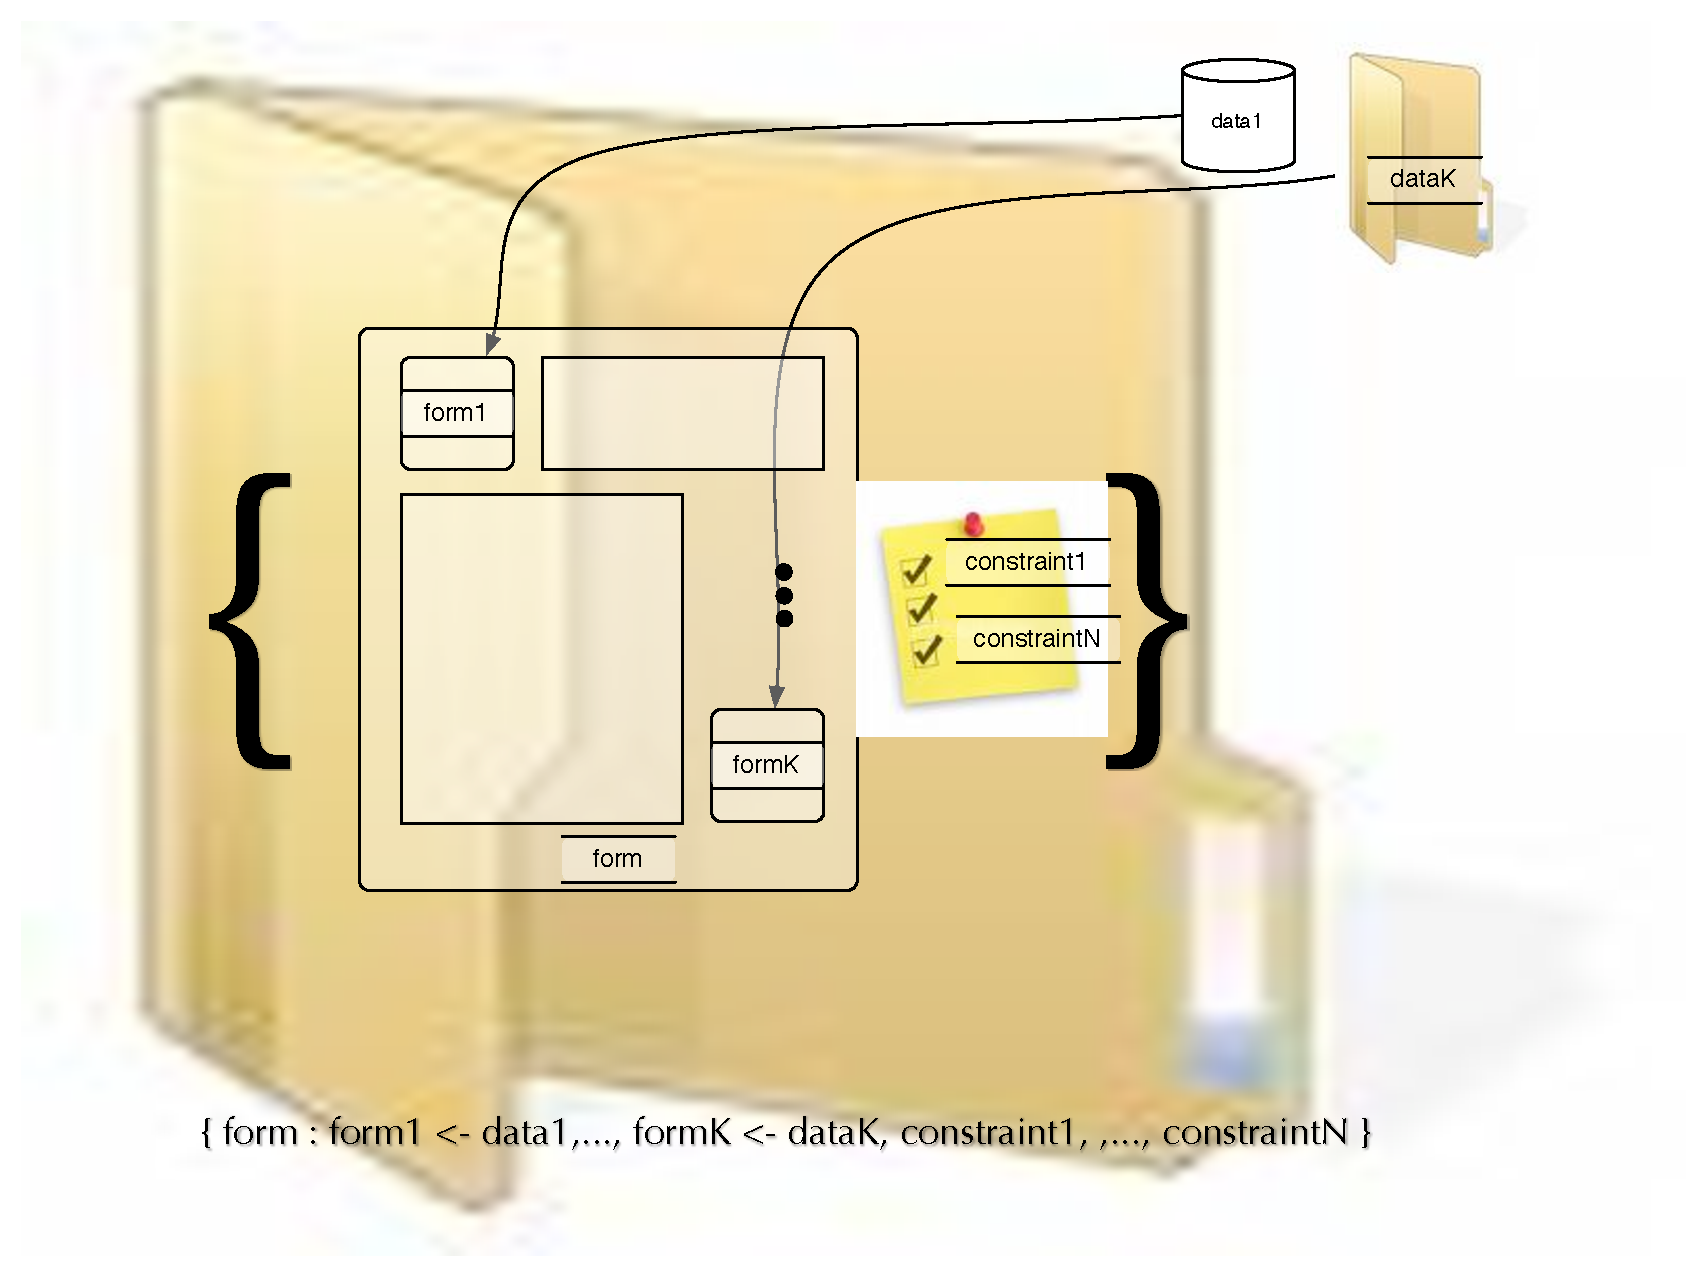
\includegraphics[scale=.65]{/Users/lgm/work/src/projex/biosimilarity/trace/src/main/book/content/figures/MonadVisualization.pdf} }
\caption{ Comprehensions and distributive maps }
\end{center}
\end{figure}


\subsubsection{Logical semantics}

\begin{mathpar}
  \inferrule* [lab=expression] {} {{c,d} ::=}
  \and
  \inferrule* [lab=identity verity] {} {\meaningof{true} = L(m)}
  \and
  \inferrule* [lab=negation] {} {\;| \; \meaningof{\neg c}= L(m) \backslash \meaningof{c}}
  \and
  \inferrule* [lab=conjunction] {} {\;| \; c \& d = \meaningof{c} \cap \meaningof{d}}
  \\
  \inferrule* [lab=mention] {} {\; | \; \bf{x} = \{ m \in L(m) \;|\: m \equiv x \}}
  \and
  \inferrule* [lab=abstraction] {} {\;| \; \meaningof{\texttt{(} \bf{x_1} \texttt{,} ... \texttt{,} \bf{x_k} \texttt{)} \; \texttt{=>} \; c} = \{ m \in L(m) \;|\; m \equiv (x_1, ..., x_k) => m', m' \in \meaningof{c} \}}
  \and
  \inferrule* [lab=application] {} {\;| \; \meaningof{c\texttt{(} c_1 \texttt{,} ... \texttt{,} c_k \texttt{)}} = \{ m \in L(m) \;|\; m \equiv m'(m_1,...,m_n), m' \in \meaningof{c}, m_i \in \meaningof{c_i} \}}
  \\
  \inferrule* [lab=let] {} {\;| \; \texttt{\bf{val}} \; \bf{x} \; \texttt{\bf{=}} \; c \texttt{;} d}
  \and
  \inferrule* [lab=seq] {} {\;| \; c \texttt{;} d }
  \and
  \inferrule* [lab=group] {} {\;| \; \texttt{ \{ } c \texttt{ \} } }
  \\
  \inferrule* [lab=probe] {} {\;| \; \meaningof{\langle d \rangle c} = \{ m \in L(m) \; | \; \exists m' \in \meaningof{d}. m'(m) \to m'', m'' \in \meaningof{c} \} }
\end{mathpar} 

\subsubsection{Other collection monads, other logics}

\paragraph{Stateful collections}

\subsection{Other logical operations}

\begin{mathpar}
  \inferrule* [lab=expression] {} {{c,d} ::=}
  \and
  \inferrule* [lab=previous] {} {\;| \; ... }
  \and
  \inferrule* [lab=quantification] {} {\;| \; \forall v . c }
  \and
  \inferrule* [lab=fixpt defn] {} {\;| \; rec \; X . c }
  \and
  \inferrule* [lab=fixpt mention] {} {\;| \; X }
\end{mathpar} 
